\appendix

\section{Online Data Contracts and Ownership}
\label{app:data-contracts}

\subsection{Canonical Online Schemas}

All online objects are versioned, immutable after emission, and validated against an allowlist
before storage. Table~\ref{tab:appendix-schemas} defines the minimum contract. Optional fields
may be absent but cannot change the meaning of a required field.

\begin{table*}[t]
\caption{Canonical online schema registry.}
\label{tab:appendix-schemas}
\centering
\scriptsize
\begin{tabular}{p{0.15\textwidth}p{0.17\textwidth}p{0.42\textwidth}p{0.17\textwidth}}
\toprule
\textbf{Object} & \textbf{Key} & \textbf{Required content} & \textbf{Permitted optional content} \\
\midrule
NormalizedEvent & \texttt{event\_id} & UTC event/ingest times; source family/instance; canonical subject, object, action; raw pointer; dependency group; schema/parser versions & source-native attributes on an explicit allowlist \\
SourceCoverage & source instance plus interval start & interval end; expected flag; health enum; observed lag; reason code; monitor/policy versions & authenticated diagnostic reference \\
EpisodeRevision & episode ID plus revision number & ordered events/links; lineage; state; fixed first-finalized time/deadline; watermark; policy version; membership digest & accepted-late reason and predecessor \\
LateEvidenceRecord & episode ID plus latest revision & beyond-horizon event/pointer; arrival/deadline; dependency root; reason; digest & none \\
FeatureVector & episode ID plus revision number & $D,C,m,o^{det}$; feature version; normalizer hashes; ordered input references & none \\
SupportDecision & episode ID plus revision number & resolved $a^{det}$; $\kappa$; group key; eligibility; manifest digest; coverage references & none \\
AuditRecord / AssemblyFailureRecord & episode ID plus revision number & complete joined outputs / terminal failure code and observed inputs; canonical digest & non-canonical runtime envelope \\
\bottomrule
\end{tabular}
\end{table*}

NormalizedEvent is produced only by Evidence Fabric; SourceCoverage only by Health Monitor;
EpisodeRevision and LateEvidenceRecord only by Episode Synthesis; FeatureVector only by Feature
Extractor; $z$ only by Stateless Scorer; SupportDecision only by Scope Resolver; $P$ only by
Calibrator; $U$ only by Sufficiency Evaluator; and AssemblyOutcome only by AuditRecord Assembler.
The store is only a sink:
it grants \texttt{INSERT} and \texttt{SELECT} but denies \texttt{UPDATE} and \texttt{DELETE} for every
emitted revision and record. A correction is represented by a new revision and record that
references its predecessor.

\subsection{Types, Time, Pointers, and Enums}

Identifiers are non-empty UTF-8 strings scoped by their producer version. Event and ingest
times are UTC RFC~3339 timestamps with microsecond precision. Raw pointers contain an
immutable object identifier, content digest, byte range or record locator, and storage schema
version; they never embed mutable file paths as identity. Health is one of
\{\path{healthy}, \path{degraded}, \path{down}, \path{unknown},
\path{not_applicable}\}. Every evidence reference includes its root dependency group so
that forwarded or derived copies remain one observation.

\subsection{Canonical Serialization and Digest}
\label{app:canonical-serialization}

The deterministic payload uses UTF-8 RFC 8785 JSON Canonicalization Scheme bytes, including
lexicographically ordered object keys and shortest round-trip decimal encodings. Arrays use
the schema's explicit domain order. NaN and infinities are forbidden. When
$\kappa=\kappa_\varnothing$, the
serialized probability field is the JSON literal \texttt{null}; it is never omitted, zeroed,
or replaced by an estimate. The canonical digest is SHA-256 over these bytes. Wall-clock
execution time, host name, process ID, memory address, and machine-specific runtime counters
are stored as a separate non-canonical envelope and cannot affect the digest.

The supplied schema sets \path{additionalProperties} to false for every object. It lists all
required and nested types, fixes enum values, and requires \path{decision_eligible}. It is
versioned as
\path{trustepisode_online.v1.schema.json}. The AuditRecord digest include set is every required field except
\texttt{canonical\_digest}; the runtime envelope is also excluded. Included examples validate a
supported record and a null-probability unsupported record. A third example containing
\texttt{malicious\_label} is required to fail schema validation.

\subsection{Firewall Examples}

A valid minimal record contains only online-observable fields:
\begin{quote}\small\ttfamily
event\_id=edr:0042;\\
event\_time=2026-07-10T04:00:00.000000Z;\\
ingest\_time=2026-07-10T04:00:01.120000Z;\\
source=EDR; subject=proc:p7; object=file:f9;\\
action=write; raw\_ref=sha256:...;\\
dependency\_group=root:0042; parser\_version=p3.
\end{quote}
The firewall must reject the same record if it includes, for example,
\path{ability_id=T1059-001} or \path{malicious_label=1}. Rejection fails the run-level
schema test, records the offending producer, and prevents the object from entering Episode
Synthesis. Merely ignoring a forbidden field downstream is insufficient.

\section{Episode Synthesis and Revision Algorithm}
\label{app:episode-algorithm}

\begin{figure*}[t]
  \centering
  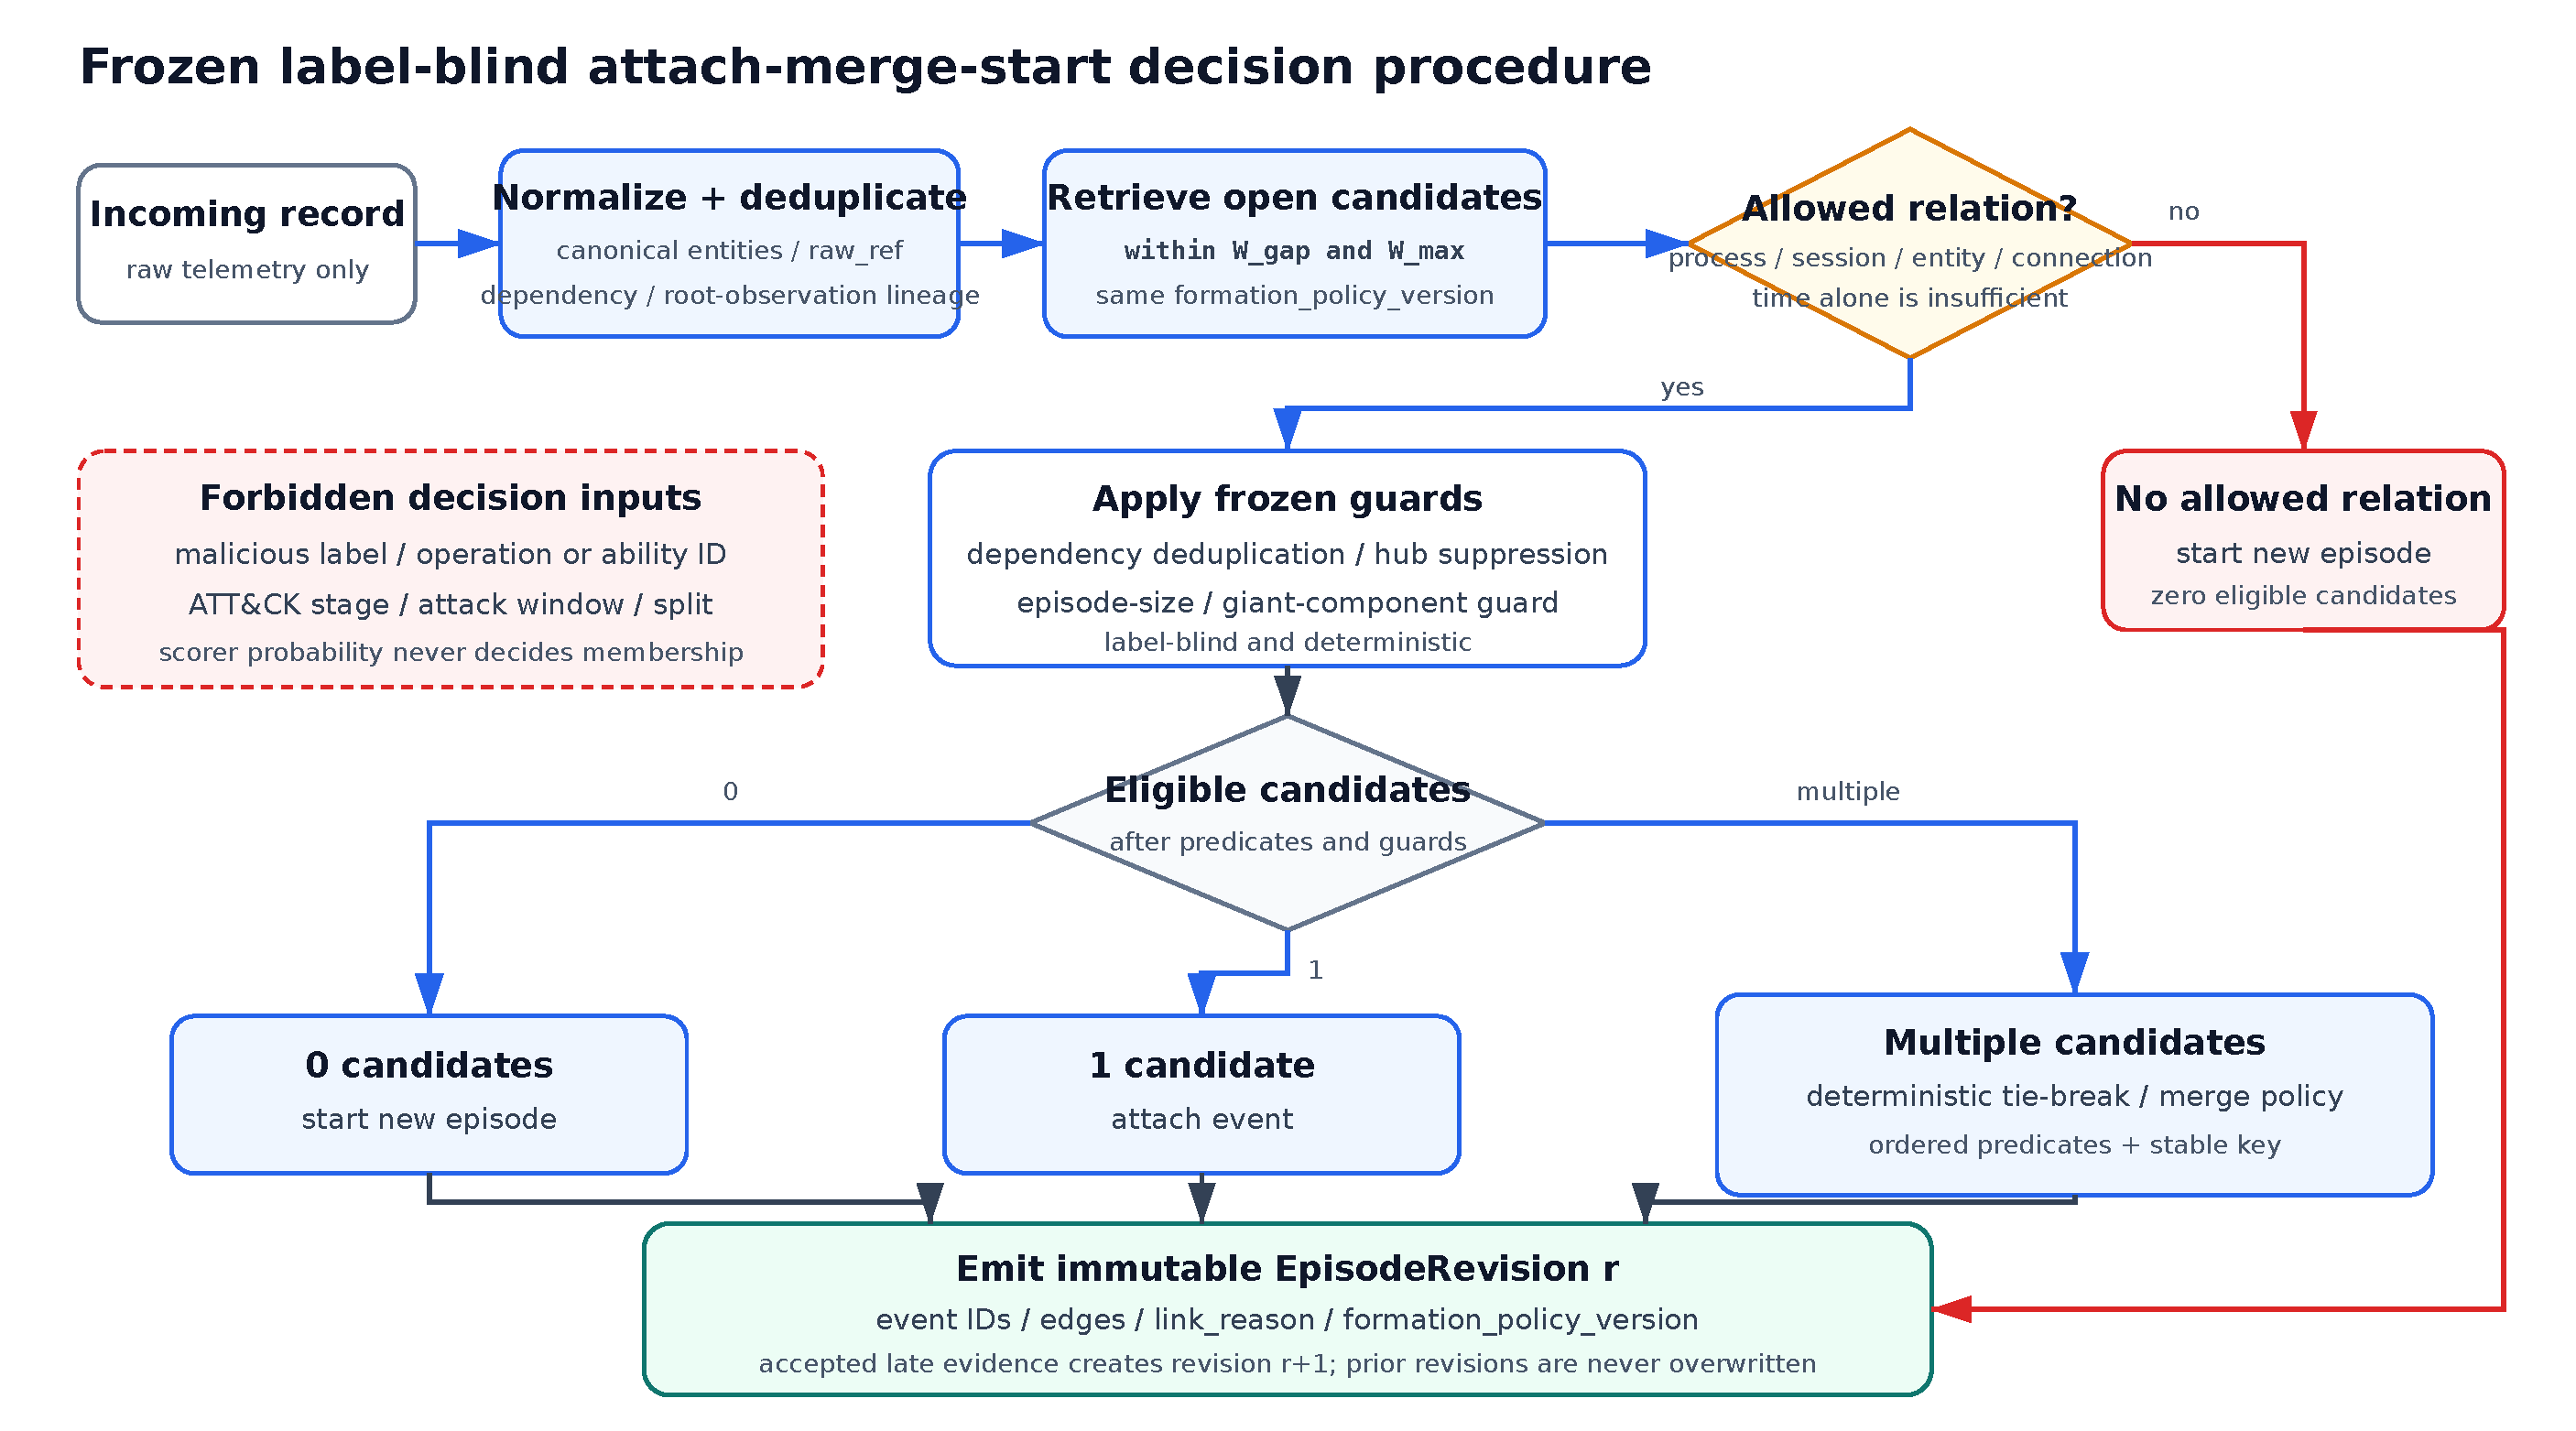
\includegraphics[width=\textwidth]{trustepisode_figures/pdf/fig08_episode_linking_decision.pdf}
  \caption{Frozen label-blind attach--merge--start procedure. Candidate retrieval, relation
  checks, guards, and total ordering execute before Episode Synthesis emits a revision; labels
  and scorer outputs cannot influence membership.}
  \label{fig:episode-linking-decision}
\end{figure*}

\subsection{Inclusive Eligibility and Allowed Relations}

Both temporal comparisons in Equation~\ref{eq:link-eligibility} are inclusive with
$W_{\mathrm{gap}}=300$ s and $W_{\max}=3600$ s:
$\Delta_t=W_{\mathrm{gap}}$ and $\operatorname{span}(E\cup\{e_i\})=W_{\max}$ remain eligible. Values larger than either bound
are ineligible. The relation predicate $R$ is true when at least one of the following frozen,
namespace-aware relations holds:
\begin{enumerate}[leftmargin=*,itemsep=1pt,topsep=2pt]
\item process parent-child or process-to-file causal continuity;
\item authenticated local/remote session continuity;
\item a network connection with a specific source/destination endpoint mapping;
\item the same non-generic host, user, process, file, service, or session entity.
\end{enumerate}
The hub predicate $H$ is true when all apparent support is attributable only to an entity with
at least 25 distinct relations in the preceding 600 s. Dependency-linked duplicates are
collapsed before $R$ and $H$ are evaluated.

\subsection{Total Order and Branch Semantics}

Candidate episodes are ordered by the tuple
\begin{equation}
(-\rho,-n_R,\Delta_t,t_{\mathrm{start}},\mathrm{episode\_id}),
\label{eq:candidate-order}
\end{equation}
where $\rho$ is the strongest relation precedence, $n_R$ is the number of distinct allowed
relation classes, $\Delta_t$ is the smallest event-time gap, $t_{\mathrm{start}}$ is episode
start time, and the final key is lexical. Relation precedence is process-causal, authenticated
session, endpoint-mapped connection, then specific-entity equality. This tuple is the only
tie-break order.

With zero eligible candidates, the builder starts an episode whose ID is the SHA-256 digest of
the formation-policy version, first event ID, and canonical namespace. With one candidate, it
attaches the event. With multiple candidates, it merges only when there are at most three
parents, every parent is connected through the new event by a process-causal, authenticated-
session, or endpoint relation, and the result has at most 500 events and 200 entities;
otherwise it attaches to the first ordered candidate. A merge ID is the digest of the literal \texttt{merge}, the sorted parent IDs, and
the formation-policy version. Parent IDs and their last revision numbers are retained as merge
lineage.

Within a revision, events are ordered by
\begin{equation}
(t^{event},t^{ingest},
\mathrm{source\_instance},\mathrm{event\_id}).
\end{equation}
The revision digest
covers the canonical episode ID, revision number, ordered membership, ordered link reasons,
lineage, and formation-policy version. These rules eliminate dependence on thread scheduling
or database return order.

\subsection{Watermark and Late Evidence}

The watermark is maximum observed ingest time minus $L_{\mathrm{wm}}=120$ s. An episode moves
\texttt{open}$\rightarrow$\texttt{finalized} when its event-time end precedes the watermark;
this freezes $t_f$ and deadline $t_f+W_{\mathrm{rev}}$. Accepted evidence before the deadline
emits a finalized successor without reopening or extending the horizon. At the deadline a
membership-identical closed successor is emitted; later evidence creates only a
LateEvidenceRecord in the late store and cannot alter history. Event time is never
overwritten to make late evidence appear timely.

\subsection{Deterministic Procedure and Replay Test}

\begin{enumerate}[leftmargin=*,itemsep=1pt,topsep=2pt]
\item Validate the NormalizedEvent schema and deduplicate by root dependency group.
\item Retrieve open episodes whose inclusive time bounds can admit the event.
\item Compute allowed relation classes and reject hub-only support.
\item Apply the 3-parent, 500-event, 200-entity, and strong-relation merge guards.
\item Sort candidates exactly by Equation~\ref{eq:candidate-order}.
\item Execute the zero/one/multiple branch and construct canonical lineage.
\item Order membership, compute the revision digest, and emit EpisodeRevision.
\item Compute $D,C,m,o^{det},z$; resolve $a^{det},\kappa,g,e$ from SourceCoverage; then compute $P,U$.
\item Join exact keys/versions and insert one AuditRecord or terminal AssemblyFailureRecord.
\item Advance the watermark; emit accepted successors or a beyond-horizon LateEvidenceRecord.
\end{enumerate}

The replay test runs the same normalized input twice under different worker counts and
database insertion orders. It compares episode/revision IDs, ordered memberships, link
reasons, lineage, features, scores, statuses, $U$, evidence references, and canonical digests.
Any mismatch is a correctness failure, not measurement noise.

\section{Feature, Sufficiency, and Parameter Registry}
\label{app:parameter-registry}

\subsection{Feature and Supporting-Evidence Contract}

For source family $s$, the empirical CDF artifact
$\widehat F^{\mathrm{train,benign}}_s$ is fit on training-benign detector values after source
parser validation. Ties use the right-continuous empirical CDF. The artifact records sample
count, fitting window, source contract, parser version, and content hash. Episode-level
$D_\epsilon$ is the arithmetic mean of the three greatest eligible transformed values. The
fixed top-three constant is not learned.

$q_{\epsilon,s}=1$ requires an upstream detection record with an immutable raw pointer, root
dependency group, detector-contract version, and a verified relation to an episode core entity
or edge. Coverage heartbeat, inventory, unscored raw presence, and another transport of the
same root observation are ineligible. The primary corroboration feature remains
$C=q_{\mathrm{EDR}}q_{\mathrm{NDR}}$ with fixed $K=2$.

Feature Extractor emits only health-independent \texttt{detected},
\texttt{examined\_none}, or \texttt{not\_examined}, together with $m$. Scope Resolver combines
these with the unique covering SourceCoverage interval to emit \texttt{available},
\texttt{no\_detection}, \texttt{collector\_unavailable}, \texttt{parser\_invalid}, or
\texttt{unknown}. Only the first two are support eligible; missing states force out-of-support
and are never interpreted as negative evidence.

\subsection{Complete Sufficiency Rules}

\begin{table*}[t]
\caption{Complete deterministic rules for $U$.}
\label{tab:u-registry}
\centering
\scriptsize
\begin{tabular}{p{0.14\textwidth}p{0.22\textwidth}p{0.56\textwidth}}
\toprule
\textbf{Axis} & \textbf{Value} & \textbf{Rule} \\
\midrule
coverage & unknown & first: any required health interval is missing or conflicting \\
 & unavailable & else any expected instance is down/not collected or any parser is invalid \\
 & degraded & else at least one expected instance is degraded \\
 & complete & else every expected instance is healthy and parser valid \\
\midrule
provenance & missing & first: any scored value, accepted link, membership event, or required root is unresolved \\
 & partial & else at least one optional unscored reference is absent \\
 & complete & else every required pointer and dependency root resolves \\
\midrule
lateness & late-accepted & first: this revision was created by accepted late evidence \\
 & revisable & else episode is open or finalized inside the 900 s horizon \\
 & stable & else episode is closed \\
\midrule
contradiction & present & first: CR1 endpoint binding, CR2 normalized flow direction, or CR3 process lineage conflict is true \\
 & unevaluable & else any applicable rule lacks required online input \\
 & none & else every applicable frozen online rule is false \\
\midrule
calibration & \texttt{supported\_global} & $\kappa=\texttt{supported\_global}$ \\
 & \texttt{supported\_group} & $\kappa=\texttt{supported\_group}$ \\
 & \texttt{out\_of\_support} & $\kappa=\texttt{out\_of\_support}$ \\
\bottomrule
\end{tabular}
\end{table*}

CR1 tests overlapping authenticated endpoint bindings for different hosts; CR2 tests matched
EDR socket/NDR flow initiator disagreement after direction normalization; CR3 tests conflicting
parent/root lineage for one $(host,boot,pid,start)$ key. A rule is applicable only when its
relation exists; missing required fields then yield \texttt{unevaluable}, while no applicable
relation yields \texttt{none}. These rules cannot read a Caldera operation, ability, attack
window, scenario, split, or offline label. The five axes are never converted to one number.

\begin{figure*}[t]
  \centering
  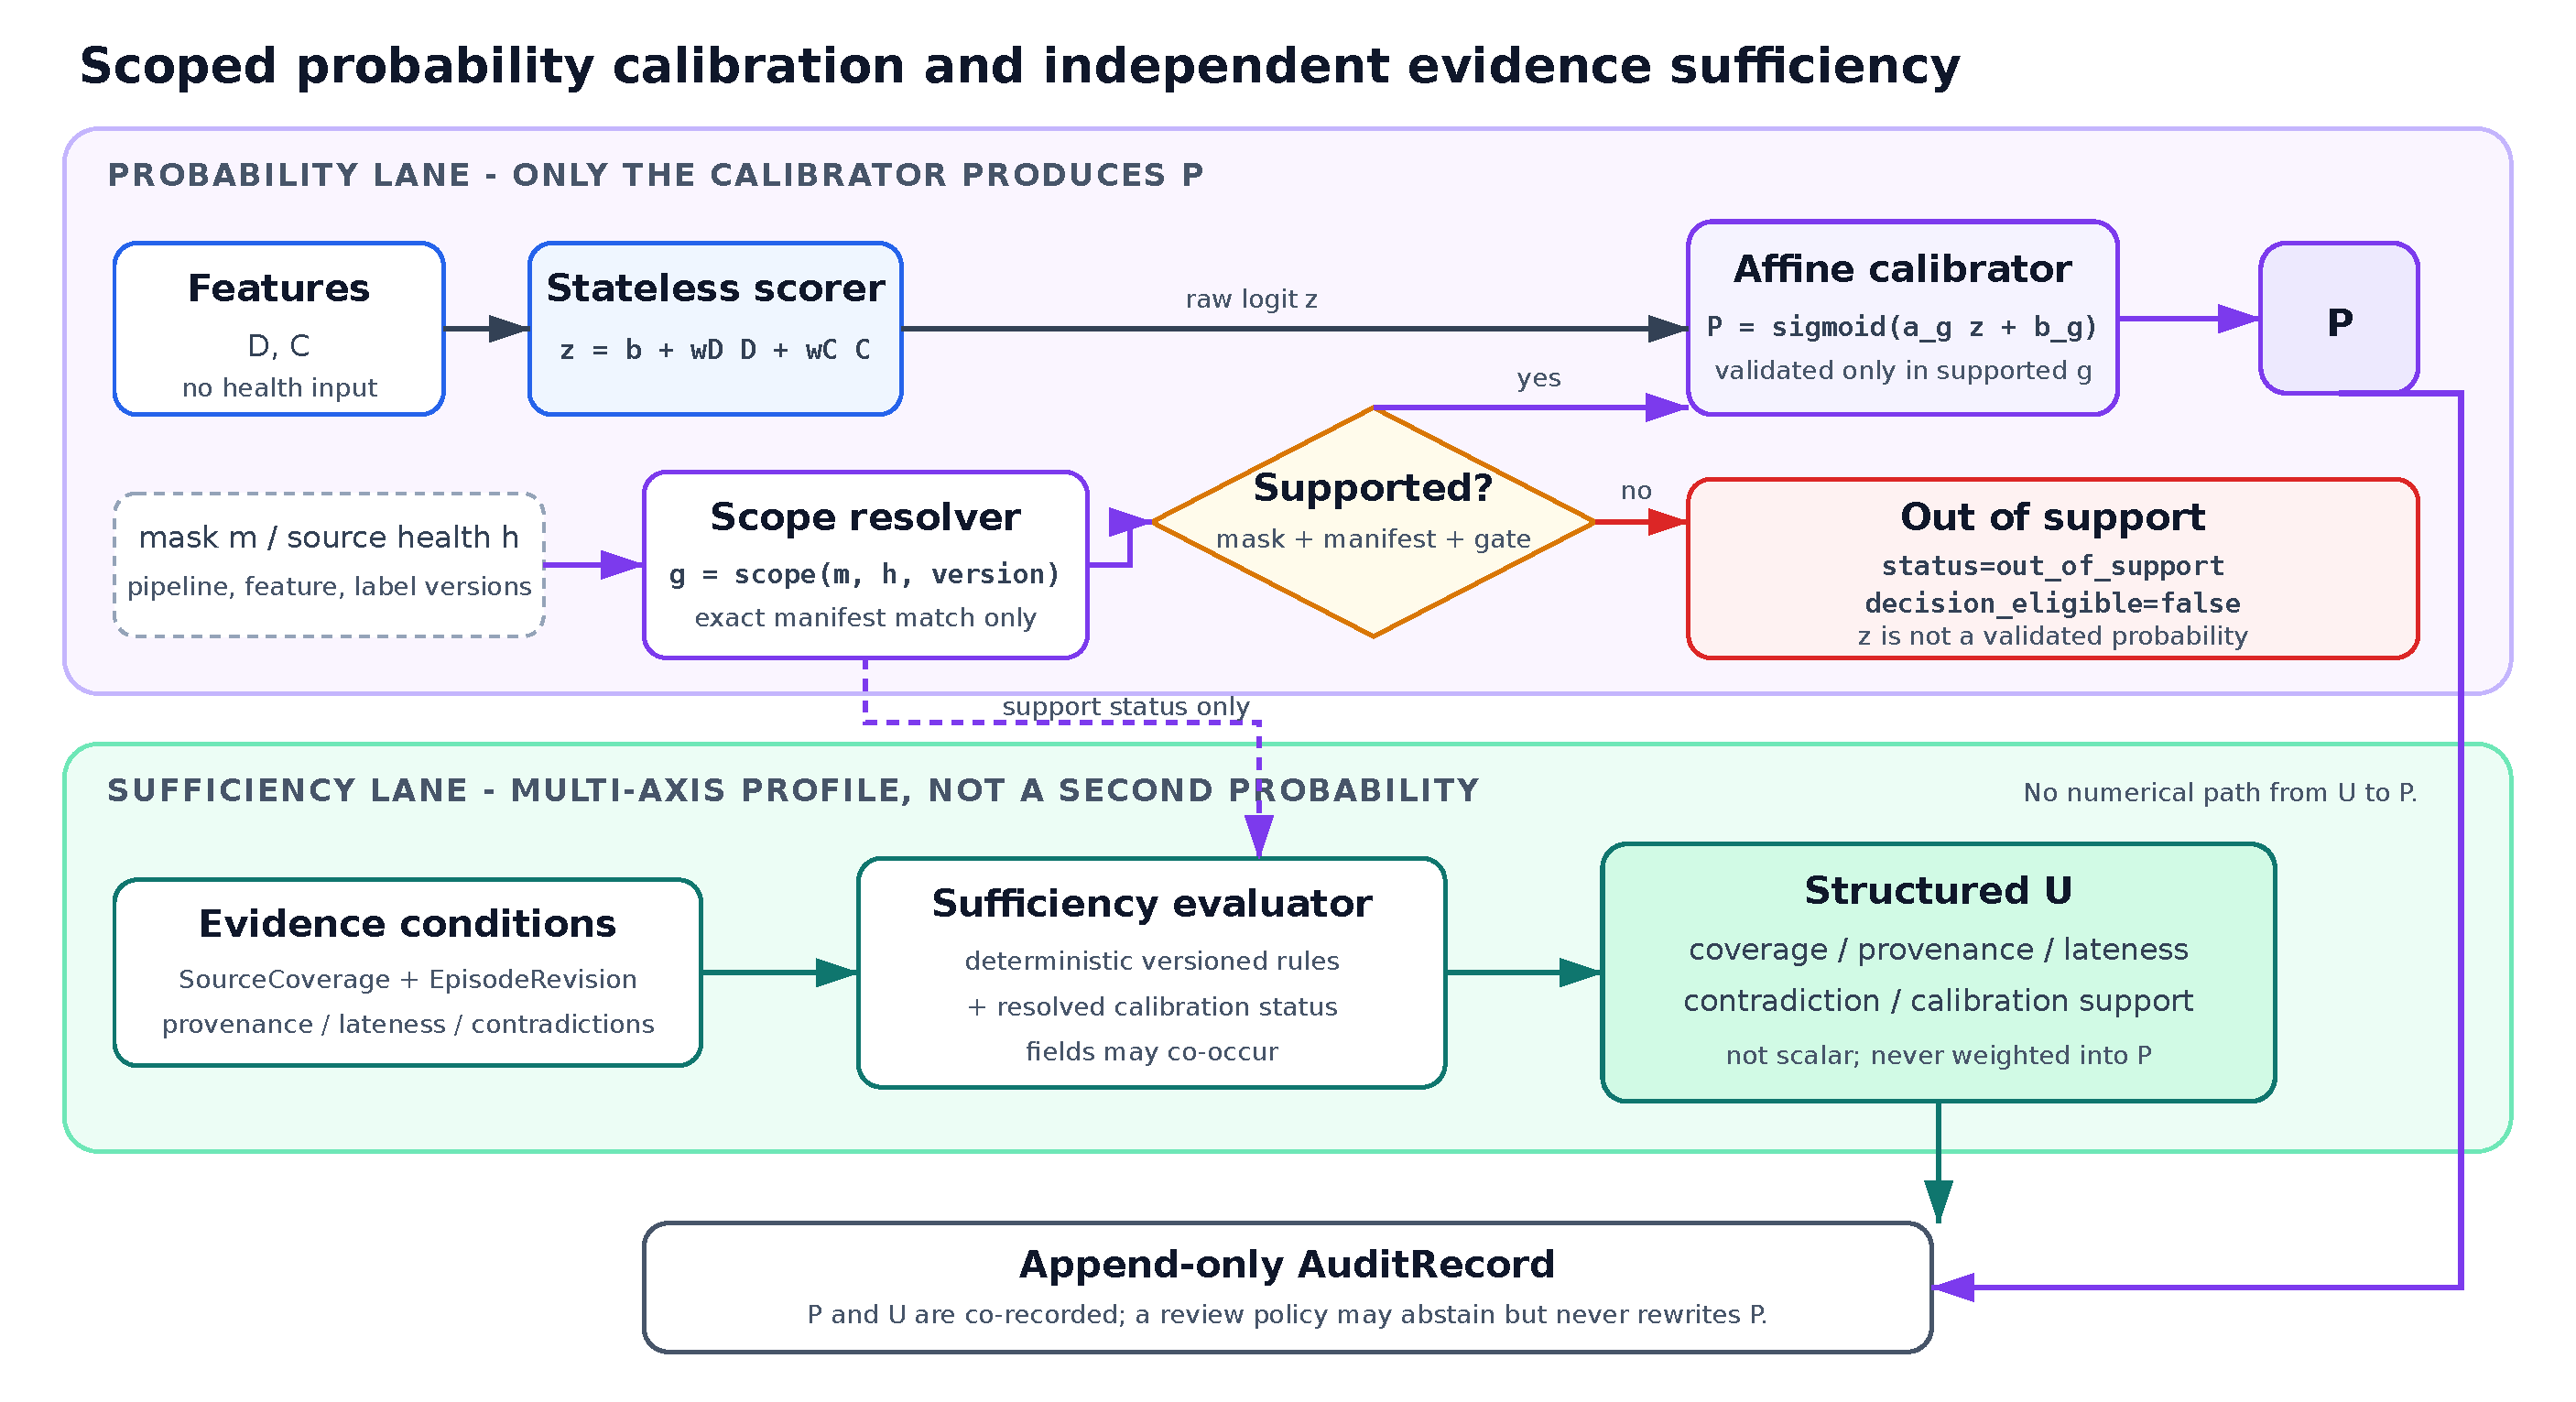
\includegraphics[width=\textwidth]{trustepisode_figures/pdf/fig03_calibration_and_sufficiency.pdf}
  \caption{Probability calibration and evidence sufficiency are independent lanes. Detector
  state participates in support resolution, while $U$ has no numerical path into $P$; the
  AuditRecord Assembler emits one terminal AssemblyOutcome to a sink-only store.}
  \label{fig:calibration-sufficiency-companion}
\end{figure*}

\subsection{Parameter Taxonomy}

\begin{table*}[t]
\caption{Parameter and state taxonomy.}
\label{tab:parameter-taxonomy}
\centering
\scriptsize
\begin{tabular}{p{0.13\textwidth}p{0.17\textwidth}p{0.07\textwidth}p{0.13\textwidth}p{0.16\textwidth}p{0.16\textwidth}}
\toprule
\textbf{Category} & \textbf{Content} & \textbf{Learned?} & \textbf{Owner} & \textbf{Selection/fit data} & \textbf{Freeze point} \\
\midrule
Scorer coefficients & $(b,w_D,w_C)$ & yes & Stateless Scorer & training fit; development selects contract & before calibration \\
Global calibrator & $(a,b_{\mathrm{cal}})$ & yes & Calibrator & natural-prevalence calibration split & before locked test \\
Conditional calibrator & $(a_g,b_g)$ & yes & Calibrator & calibration run folds after gate & before locked test \\
Formation policy & time, revision, hub, component, merge settings & no & Episode Synthesis & training/development & before final train-only fit \\
Fixed aggregation & top three; primary $K=2$ & no & Feature contract & method specification & before training \\
Evidence state & $m,h,q,a^{det}$ & no & Table~\ref{tab:ownership} producers & runtime observation & per revision \\
Output/status & $\kappa,U$ & no & Scope/Sufficiency Evaluators & deterministic runtime rules & per AuditRecord \\
Version metadata & schema, policy, model, calibrator, manifest hashes & no & Artifact Registry & producing artifact's split & artifact publication \\
Evaluation settings & split seed, perturbations, bootstrap repetitions & no & Evaluation Harness & pilot/development preregistration & before locked test \\
\bottomrule
\end{tabular}
\end{table*}

The unconditional primary method therefore has five fitted scalar coefficients:
$\{b,w_D,w_C,a,b_{\mathrm{cal}}\}$. Empirical CDFs are frozen fitted preprocessing artifacts,
not fixed constants. Conditional group coefficients exist only for groups that pass the
registered gate.

\subsection{Single Threshold Registry}

Every threshold is defined only in Table~\ref{tab:threshold-registry}; other sections refer to
its symbol and owner.

Primary values are $W_{\mathrm{gap}}=300$ s, $W_{\max}=3600$ s,
$W_{\mathrm{rev}}=900$ s, $L_{\mathrm{wm}}=120$ s, $f_{\mathrm{hub}}=25$ distinct
relations per 600 s, and $n_{\mathrm{component}}=(500\text{ events},200\text{ entities})$.
Label/matching values are $\theta_{\mathrm{mal}}=.50$,
$\theta_{\mathrm{contam}}=.25$, and $\theta_{\mathrm{match}}=.50$ with minimum time IoU .10
and entity Jaccard .50. The group gate fixes
$(n_{\mathrm{pos}}^{\min},n_{\mathrm{neg}}^{\min},n_{\mathrm{run}}^{\min})=(50,50,10)$,
five run folds, and minimum mean Brier/NLL improvements $(.01,.01)$ with positive paired 95\%
lower bounds. Values are mirrored in \path{thresholds.v1.json}; a code/paper mismatch fails
artifact validation.

\begin{table*}[t]
\caption{Threshold ownership, selection, freeze, and validation registry.}
\label{tab:threshold-registry}
\centering
\scriptsize
\begin{tabular}{p{0.12\textwidth}p{0.25\textwidth}p{0.17\textwidth}p{0.16\textwidth}p{0.20\textwidth}}
\toprule
\textbf{Symbol} & \textbf{Meaning} & \textbf{Owner} & \textbf{Selection data} & \textbf{Freeze and validation} \\
\midrule
$W_{\mathrm{gap}}$ & maximum event-time inactivity gap & formation policy & development & before final train fit; EB1/EB2 sensitivity \\
$W_{\max}$ & maximum event-time episode span & formation policy & development & before final train fit; M7 sensitivity \\
$W_{\mathrm{rev}}$ & post-watermark revision horizon & revision policy & development/pilot & before calibration; delay replay \\
$L_{\mathrm{wm}}$ & allowed ingest lateness for watermark & revision policy & development/pilot & before calibration; delay replay \\
$f_{\mathrm{hub}}$ & generic/high-frequency entity cutoff & formation policy & training/development & before final train fit; EB3-H ablation \\
$n_{\mathrm{component}}$ & giant-component event/entity limit & formation policy & development & before final train fit; stress replay \\
$\theta_{\mathrm{mal}}$ & minimum malicious overlap for positive label & label policy & pilot/adjudication & before partitioned labels are released \\
$\theta_{\mathrm{contam}}$ & unrelated-benign overlap for mixed label & label policy & pilot/adjudication & before partitioned labels are released \\
$n_{\mathrm{pos}}^{\min}$ & minimum group-calibration positives & calibration gate & pre-registered before calibration & before group fitting; internal run folds \\
$n_{\mathrm{neg}}^{\min}$ & minimum group-calibration negatives & calibration gate & pre-registered before calibration & before group fitting; internal run folds \\
$n_{\mathrm{run}}^{\min}$ & minimum independent calibration runs & calibration gate & pre-registered before calibration & before group fitting; internal run folds \\
$\Delta_{\mathrm{miscal}}^{\min}$ & minimum validated global-calibration deficiency & calibration gate & pre-registered before calibration & internal run folds only \\
$\theta_{\mathrm{match}}$ & minimum action/entity overlap for episode matching & evaluation policy & development & before locked test; matching sensitivity \\
\bottomrule
\end{tabular}
\end{table*}

\section{Calibration Manifest, Eligibility, and Invalidation}
\label{app:calibration-manifest}

\subsection{Manifest Contract}

\begin{table*}[t]
\caption{Required calibrator-manifest fields.}
\label{tab:calibrator-manifest}
\centering
\scriptsize
\begin{tabular}{p{0.26\textwidth}p{0.63\textwidth}}
\toprule
\textbf{Field group} & \textbf{Required values} \\
\midrule
Candidate contract & formation-policy version; candidate-selection version; label-policy version \\
Feature contract & feature version; EDR/NDR detector-contract versions; empirical-CDF hashes; detector-state and missing-value contract \\
Model contract & raw-model version and digest; coefficient digest; training split manifest \\
Calibration contract & calibrator version; global coefficients; registered group-key fields/digests; eligible final-refit coefficients; calibration split manifest \\
Runtime support & exact source mask \texttt{11}; allowed health/detector states; schema/parser versions; deployment/pipeline version \\
Evidence and audit & calibration counts, prevalence as metadata, gate evidence, reliability-bin specification, manifest digest \\
\bottomrule
\end{tabular}
\end{table*}

Support requires exact equality for every contract field that affects candidate construction,
features, raw scores, or calibration meaning. The resolver never chooses a nearest source mask
or silently maps a novel pipeline version to an old artifact.

\subsection{Global and Conditional Group Resolver}

The global mapping uniquely minimizes natural-prevalence NLL plus
$10^{-6}(a^2+b_{\mathrm{cal}}^2)$ subject to $a\ge10^{-6}$. Primary support requires exact
mask \texttt{11}, no down/unknown health, valid parsers, and detector states
\texttt{available} or \texttt{no\_detection}. Each group key is pre-registered as the RFC~8785/
SHA-256 digest of deployment profile and EDR/NDR detector versions; scenario, run, identity,
and label fields are forbidden. A group is considered only with
at least 50 positives, 50 negatives, and 10 independent runs. Runs use deterministic five-fold
assignment with seed 20260710; each fold evaluates a mapping fitted on the other four. A group
is enabled only when mean held-out improvements in both Brier and NLL are at least .01, every
fold is nonnegative, and both paired run-bootstrap lower 95\% bounds exceed zero. Undefined or
tied gates fall back to global. Passing group coefficients are then refit on all calibration
records for the exact key and sealed in a duplicate-key-rejecting manifest; locked test never
selects or refits a group.

Resolution follows one exclusive branch:
\begin{enumerate}[leftmargin=*,itemsep=1pt,topsep=2pt]
\item Exact support plus one enabled exact group key:
      use $(a_g,b_g)$ and serialize \path{supported_group}.
\item Exact support without an enabled exact key:
      use $(a,b_{\mathrm{cal}})$ and serialize \path{supported_global}.
\item Any required manifest or supported-regime mismatch:
      serialize \path{out_of_support}, set $P=\texttt{null}$, and set
      \path{decision_eligible=false}.
\end{enumerate}
Group-gate failure is therefore distinct from out-of-support status.

\begin{figure*}[t]
  \centering
  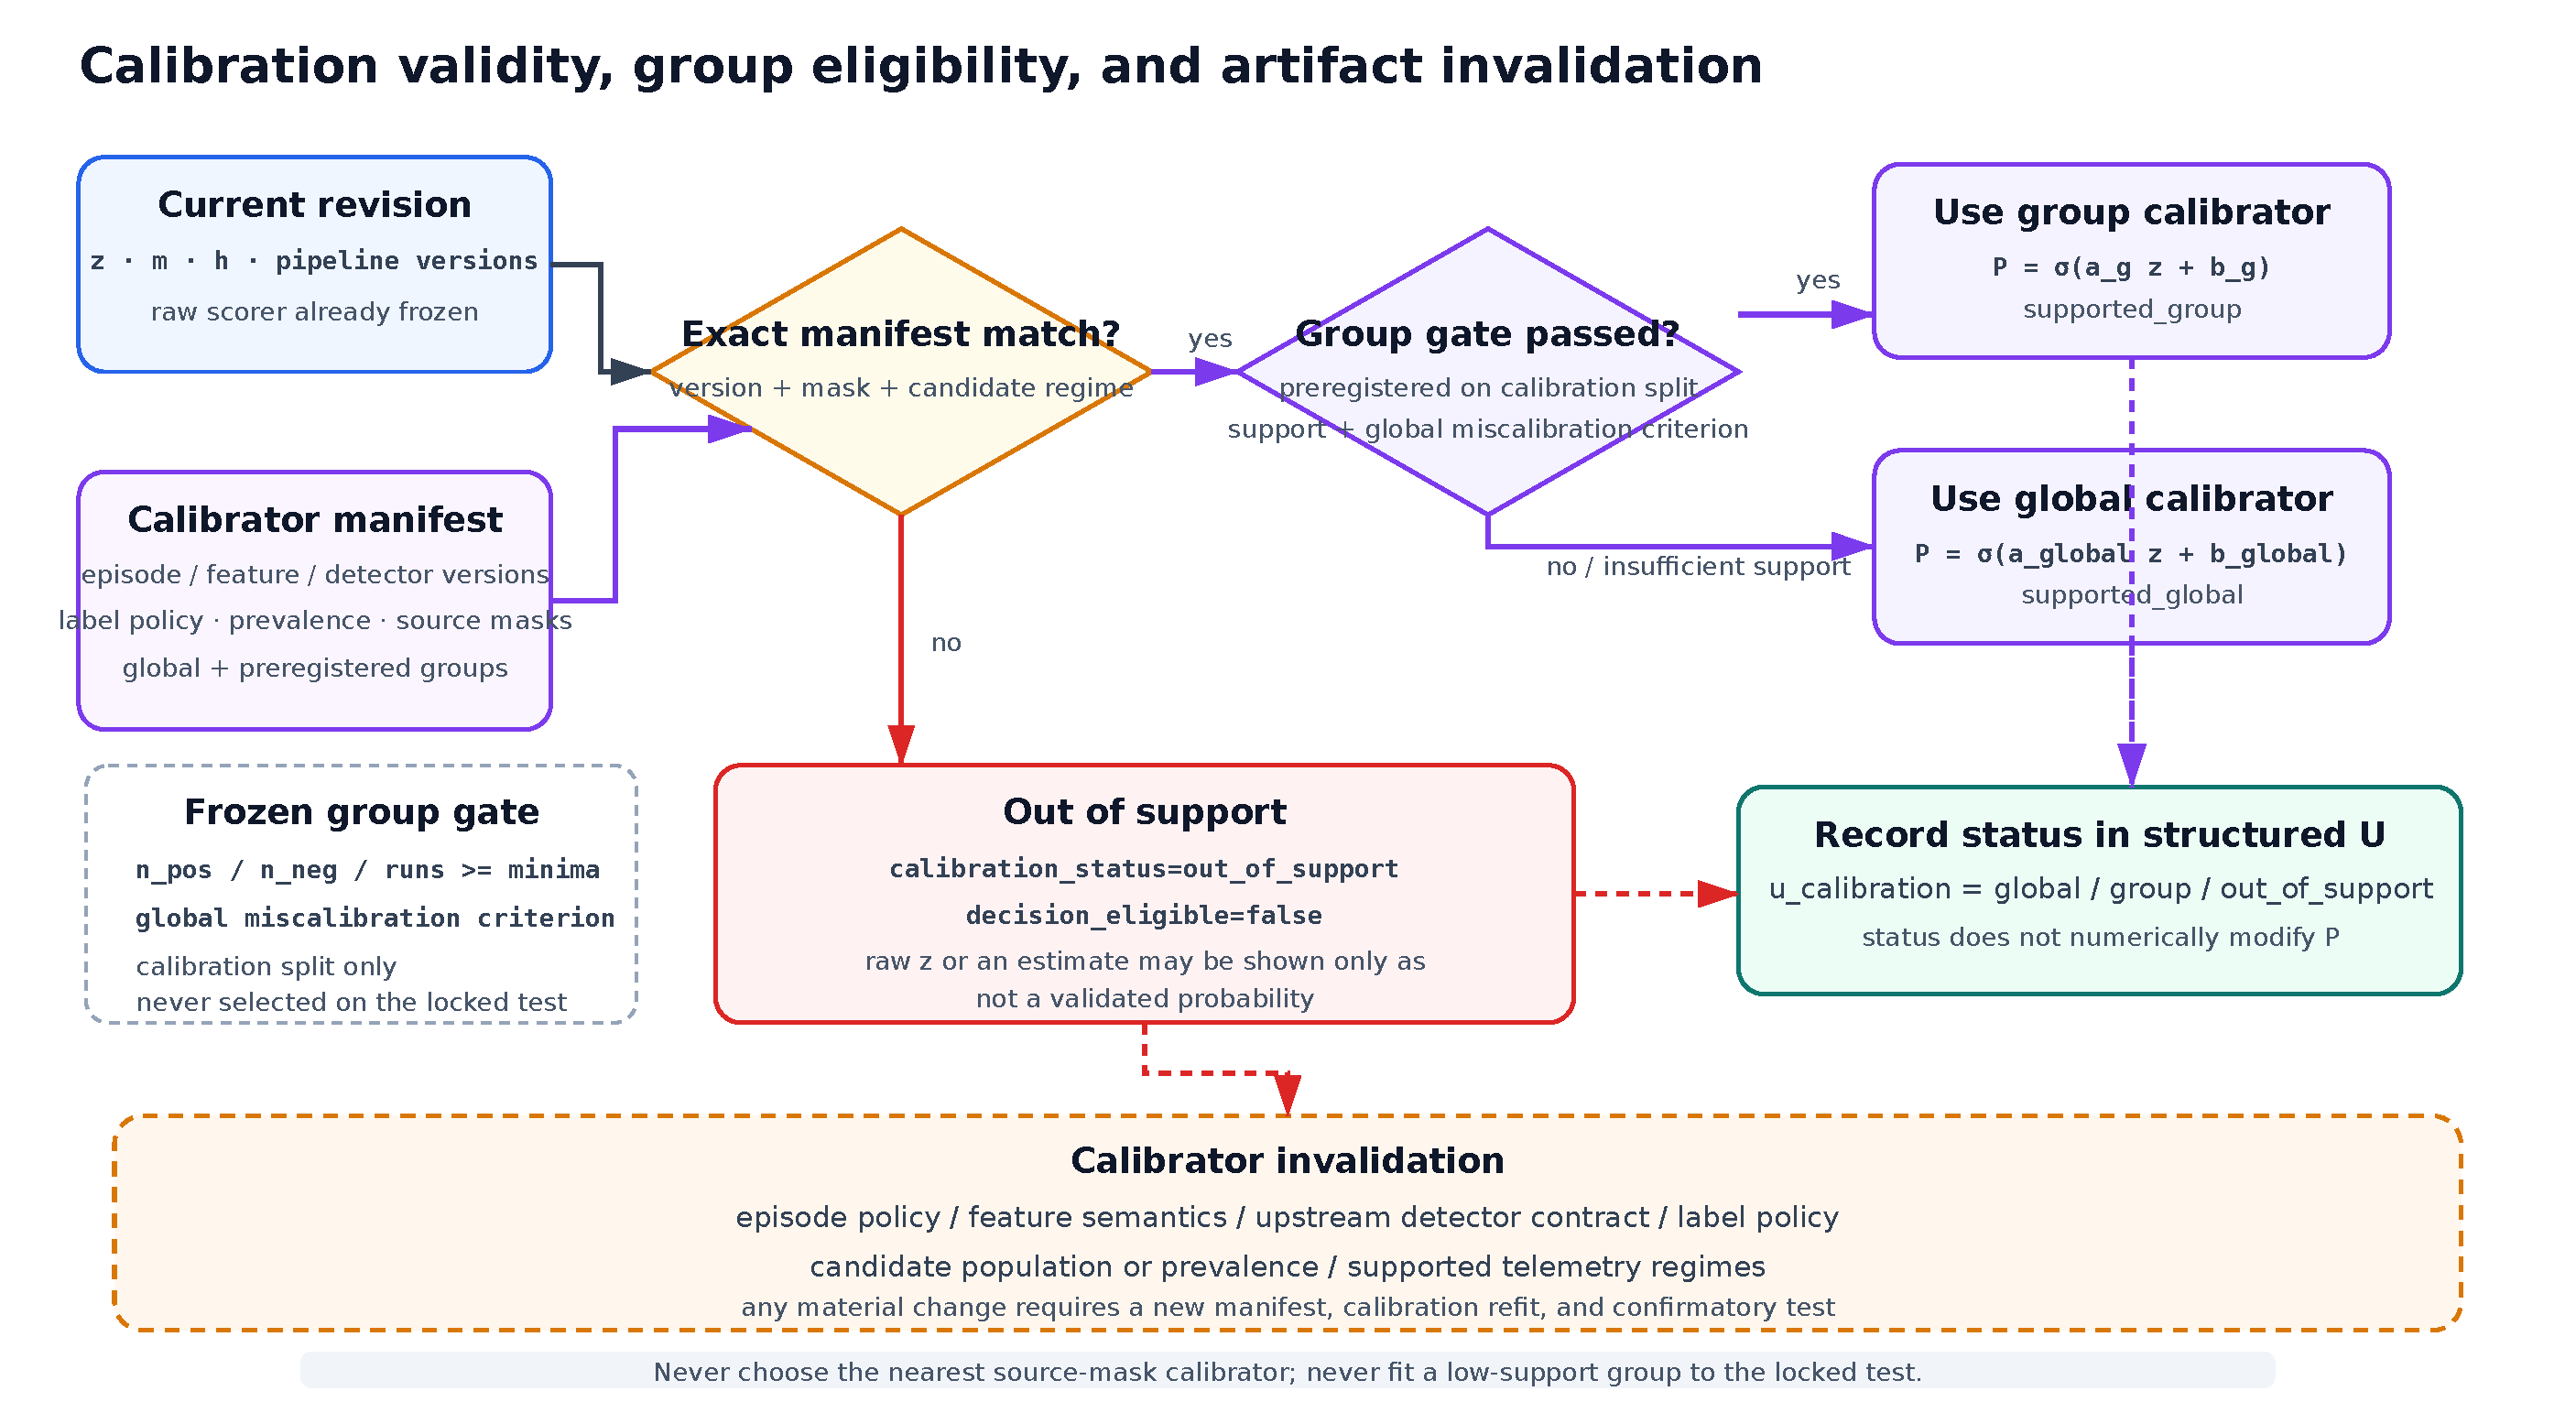
\includegraphics[width=\textwidth]{trustepisode_figures/pdf/fig09_calibration_validity_state_machine.pdf}
  \caption{Exclusive calibration resolution and invalidation. Exact source, health, detector,
  and version support is required; the five-fold group gate can only select between a
  registered group and global fallback, never manufacture support.}
  \label{fig:calibration-validity-companion}
\end{figure*}

\subsection{Invalidation Matrix}

\begin{table*}[t]
\caption{Calibrator invalidation and revalidation rules.}
\label{tab:calibrator-invalidation}
\centering
\small
\begin{tabular}{p{0.29\textwidth}p{0.30\textwidth}p{0.31\textwidth}}
\toprule
\textbf{Change} & \textbf{Immediate status} & \textbf{Required action} \\
\midrule
Episode policy or candidate-selection policy & invalid & rebuild candidates; refit scorer and calibrator \\
Feature semantics, normalizer, or missing rule & invalid & refit scorer and calibrator \\
Upstream detector contract or parser semantics & out of support & revalidate features; refit if distribution/meaning changes \\
Raw-model coefficients or training population & invalid & refit calibrator \\
Label policy & invalid for supervised claim & regenerate labels; repeat fit and evaluation \\
Supported source mask or health regime & out of support & collect calibration support and register a new manifest \\
Schema-only additive field excluded from features & pending compatibility check & prove canonical equivalence before manifest amendment \\
Candidate prevalence drift & revalidation signal only & audit reliability; do not automatically change episode-level output \\
\bottomrule
\end{tabular}
\end{table*}

Prevalence is recorded because it affects interpretation and may motivate revalidation, but an
unknown current deployment prevalence is never an online per-revision gate. Out-of-support
records expose $z$ only with raw-logit wording and serialize $P$ as canonical null under
Appendix~\ref{app:canonical-serialization}.

\section{Laboratory, Ground Truth, and Label Policy}
\label{app:lab-label-policy}

\subsection{Run and Environment Manifest}

Every formal run stores: run and pair IDs; scenario and benign-workload manifest versions;
Caldera v5.3.0 annotated tag object
\texttt{dd22d543a519afe63ca35c454bf1add5d75c45dc}, peeled commit
\texttt{b24f6e7a99cab19cbf417009bda9b9c6c81abc31}; target image SHA-256 hashes;
VM and network topology versions;
EDR/NDR collector images and configuration hashes; Health Monitor version; parser/schema
versions; clock source and maximum observed skew; random seed; start/end times; harmless
marker IDs; cleanup status; and any collection incident. Formal evaluation has no public-data
tier: provenance datasets remain related-work context because they do not implement the frozen
EDR/NDR collection contract. Formal results group by this run ID, not by Caldera ability or
individual episode. The complete machine contract is
\path{artifacts/contracts/lab_manifest.v1.json}; a missing required field fails closed.

\begin{figure*}[t]
  \centering
  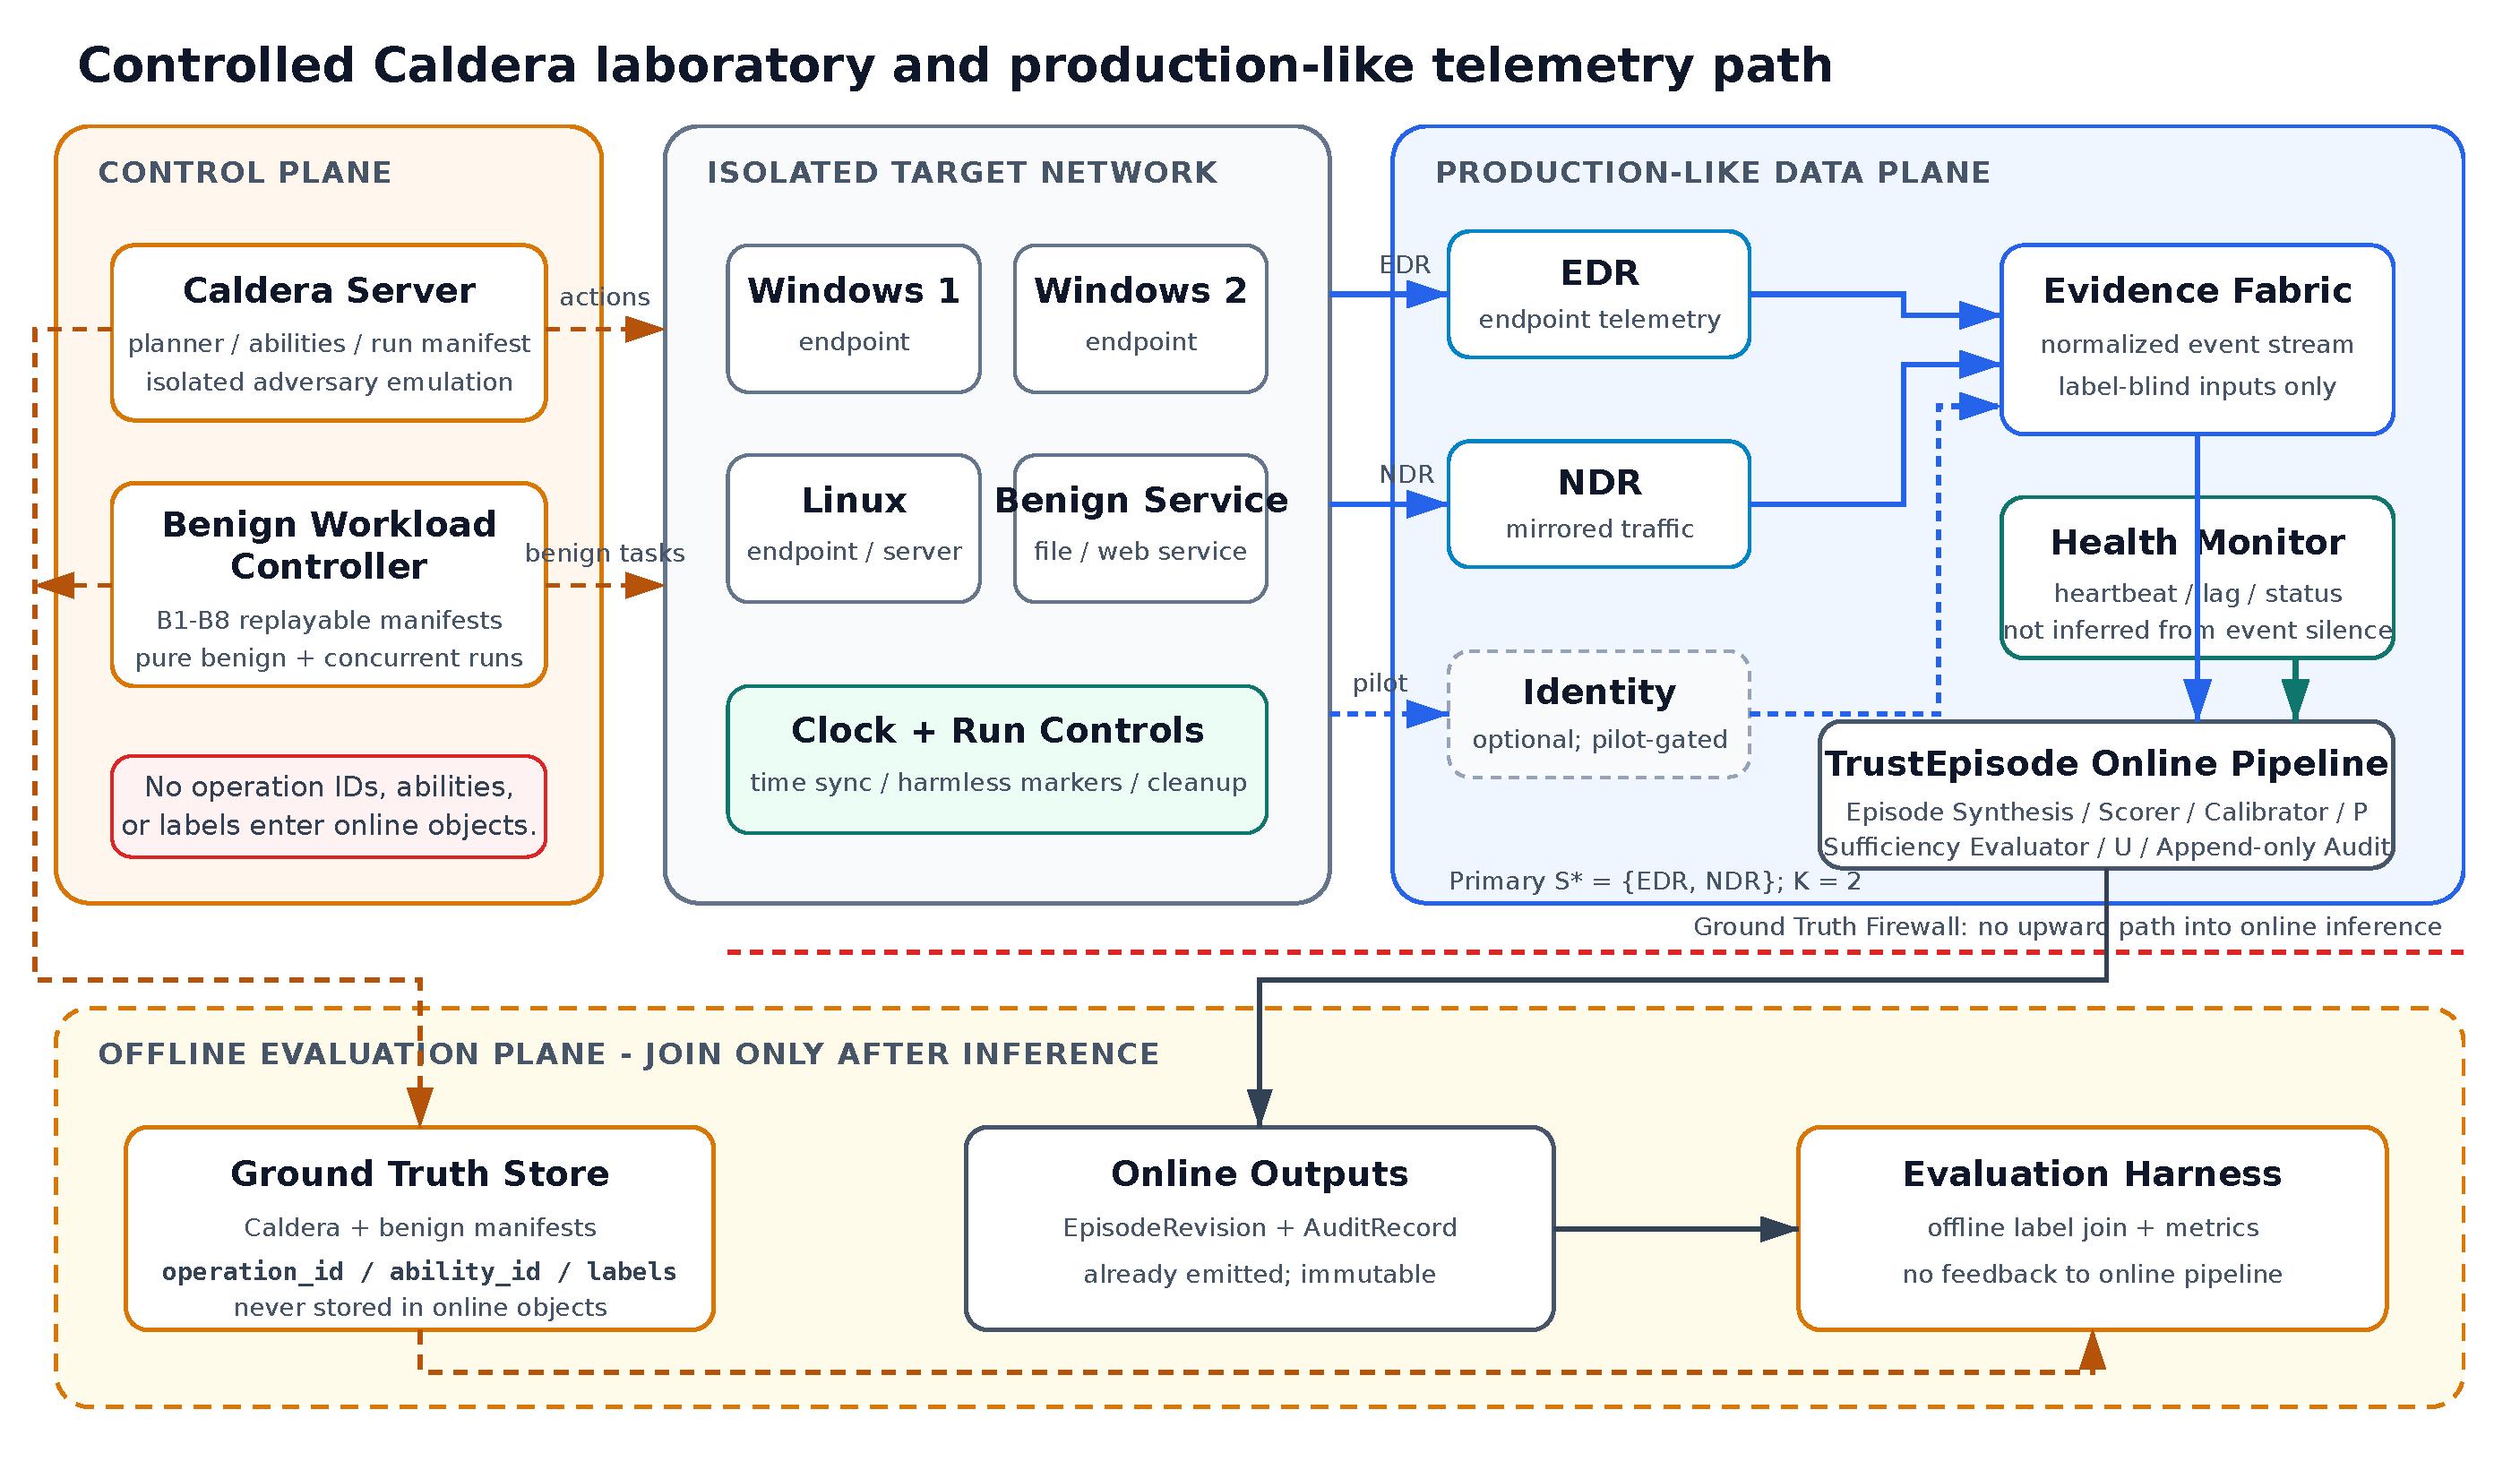
\includegraphics[width=\textwidth]{trustepisode_figures/pdf/fig04_lab_topology.pdf}
  \caption{Controlled laboratory topology. EDR and NDR are the only online telemetry sources;
  Identity is excluded from the candidate path and M5-ID can join only in offline evaluation.}
  \label{fig:lab-topology-companion}
\end{figure*}

\subsection{Scenario Cards and Failure Rules}

\begin{table*}[!t]
\caption{Malicious scenario-card registry. Actions use only isolated targets and harmless
per-run markers.}
\label{tab:scenario-cards}
\centering
\scriptsize
\begin{tabular}{p{0.05\textwidth}p{0.34\textwidth}p{0.28\textwidth}p{0.23\textwidth}}
\toprule
\textbf{ID} & \textbf{Precondition and ordered actions} & \textbf{Marker and expected observations} & \textbf{Cleanup and card-specific failure} \\
\midrule
M1 & two Windows targets and test share; discovery $\rightarrow$ share access $\rightarrow$ test-account remote execution & unique process/file marker; EDR lineage plus NDR remote connection & remove marker/session/service; abort if either primary collector fails \\
M2 & Windows target; script execution $\rightarrow$ staged marker transfer $\rightarrow$ temporary scheduled-task persistence & script/process/file marker; EDR lineage and NDR transfer & delete task and marker; record inability to remove persistence as cleanup failure \\
M3 & Linux targets; discovery $\rightarrow$ test-account SSH $\rightarrow$ marker file action & shell/file marker; Linux EDR lineage and NDR SSH flow & terminate shell, revoke key, remove marker; abort on namespace mismatch \\
M4 & instrumented service; low-rate periodic connections $\rightarrow$ local marker action & seeded connection cadence plus EDR local action & stop client and remove marker; fail card if cadence manifest is not replayed \\
M5 & test-account endpoint action $\rightarrow$ endpoint marker & EDR/NDR primary evidence independent of Identity & revoke credential and marker; fail if either primary collector is unhealthy \\
M6 & dual-use administration tool also present in benign cards; contextual misuse $\rightarrow$ remote marker action & identical tool name in both classes; sequence/context plus EDR/NDR distinguish use & remove marker/session; preserve unsuccessful execution as declared failure \\
M7 & extended schedule; discovery $\rightarrow$ frozen pauses $\rightarrow$ remote action $\rightarrow$ marker & weak observations across $W_{\mathrm{gap}}$/$W_{\max}$ boundaries & terminate sessions/markers; report any schedule-bound violation \\
\bottomrule
\end{tabular}
\vspace{8pt}
\caption{Benign and hard-negative workload-card registry.}
\label{tab:benign-cards}
\centering
\scriptsize
\begin{tabular}{p{0.05\textwidth}p{0.34\textwidth}p{0.28\textwidth}p{0.23\textwidth}}
\toprule
\textbf{ID} & \textbf{Precondition and ordered actions} & \textbf{Expected observations} & \textbf{Cleanup and card-specific failure} \\
\midrule
B1 & approved PowerShell/bash inventory over registered targets & process, query, and normal connection evidence & remove output; fail if command leaves target state changed \\
B2 & signed test patch deployment and verification & installer lineage, package writes, repository flow & uninstall/revert snapshot; record reboot or rollback failure \\
B3 & seeded file-share synchronization of benign fixtures & burst file operations and SMB/NFS flows & remove synchronized fixtures; verify checksums \\
B4 & authorized vulnerability scan against isolated service & high fan-out NDR flows and expected service logs & stop scanner; fail if target leaves healthy state \\
B5 & helpdesk test-account remote administration & same remote/admin tools used in M1/M6 without malicious marker & terminate session and revoke temporary grant \\
B6 & scheduled log collection and forwarding & repeated reads, compression, and collector-bound network flow & remove bundle; verify no collector backlog \\
B7 & configuration-management convergence to a known benign state & remote orchestration, file/service updates, expected restart & restore baseline; fail on manifest drift \\
B8 & unscheduled but declared maintenance with a frozen work order & realistic administrative sequence with healthy EDR/NDR & verify service state; retain timing as hard-negative context \\
\bottomrule
\end{tabular}
\end{table*}

Every card records its version, target images, benign mode, repetition ID, and seed. Each
malicious family has exactly 10 successful attack-only repetitions and 10 successful
concurrent-benign repetitions; B1--B8 each have exactly 10 successful pure-benign repetitions.
The machine-readable ordered actions, markers, observations, cleanup, and failure rules are in
\path{artifacts/contracts/scenario_cards.v1.json}. A collection failure excludes the run from
primary metrics but remains in RT1 and the failure log. A failed scenario action
with healthy primary collectors remains in the registered sensitivity view but not the
successful-run cohort. Cleanup failure blocks the next run on that image. No failed or aborted
run is silently reused under the same ID.

\subsection{Identity Pilot Gate}

Identity remains conditional under the separately registered M5-ID card. Before any
Identity-side analysis, pilot runs must demonstrate complete
timestamp alignment, stable benign and malicious capture, independent source health, raw
provenance pointers, and sufficient run-level support. Identity is always excluded from
NormalizedEvent, Episode Synthesis, candidate IDs and membership, $D,C,z$, every calibrator
manifest, and primary RQs. Gate failure suppresses all Identity-side reporting. Gate passage
permits only a separately labeled offline exploratory annotation after primary inference; it
cannot change the EDR/NDR candidate universe or $K=2$ contract.

\subsection{Ground Truth Store and Offline Join}

The Ground Truth Store uses a separate database role. Join keys are run ID, harmless marker
ID, target entity namespace, and versioned time interval. The Evaluation Harness first verifies
that online inference and AuditRecord insertion have completed, then performs the join under
the frozen label-policy digest. A two-reviewer adjudication resolves disagreements; unresolved
cases become ambiguous rather than being forced into the binary cohort.

Offline matching first requires temporal IoU at least $.10$, entity Jaccard at least $.50$,
and one exact harmless marker or registered action. Within one run, maximum-weight bipartite
assignment uses
$w=.5A_{cov}+.3J_{entity}+.2\operatorname{IoU}_{time}\ge\theta_{match}=.50$;
ties use entity overlap, absolute time difference, then lexical IDs. A revision is positive
when malicious-action coverage is at least $\theta_{mal}=.50$ and unrelated benign
contamination is below $\theta_{contam}=.25$; mixed when both thresholds are met; negative when
malicious coverage is zero and activity has registered benign/background attribution; all
residual, missing, or conflicting cases are ambiguous. Labels are revision specific and join
only after AuditRecord insertion. Sensitivity varies $\theta_{mal}\in\{.25,.50,.75\}$,
$\theta_{contam}\in\{.10,.25,.50\}$, and $\theta_{match}\in\{.40,.50,.60\}$ without altering
the primary registry after seeing performance.

\subsection{Leakage Tests}

Continuous schema tests inject each forbidden field into every online object and require a
hard rejection. Partition tests verify that every descendant of one run has exactly one split.
Feature-lineage tests prove that all scorer inputs trace to allowed online fields. SQL-role
tests deny online reads from Ground Truth Store tables. A canary scenario token is placed only
in the offline store and must be absent from every normalized event, revision, feature, model
input, and AuditRecord. Any failure invalidates the affected run and blocks locked evaluation.

\clearpage
\section{Experimental Contract and Reproducibility}
\label{app:experimental-contract}

\subsection{Split and Freeze Manifest}

The registered views prevent revision multiplicity from changing a claim. $\mathcal C_{form}$
contains one terminal revision per surviving lineage at
$T_{form}=t_{run\_end}+L_{wm}+W_{rev}=t_{run\_end}+1020$ s, after removing merged parents.
$\mathcal C_{dec}$ contains the first finalized, decision-eligible revision per terminal
episode and is the only primary RQ2 population. $\mathcal C_{stream}$ contains every
AuditRecord keyed by $(episode\_id,revision)$ and is used only for RQ3/RQ4 transitions and
cost.

The independent split unit is a base campaign, stratified by scenario family and benign mode.
Within each stratum, campaigns sort by ascending SHA-256 of
\texttt{20260710:base\_campaign\_id}. In each consecutive 20-run cycle, ranks 0--9 are
training, 10--13 development, 14--16 calibration, and 17--19 locked test, targeting
50/20/15/15 percent. Replay and outage descendants inherit partition and bootstrap cluster;
any mismatch invalidates the complete cluster. The registry requires run, base, parent, and
pair IDs; scenario; benign mode; seed; partition; cluster; role; and manifest digest. The
freeze manifest additionally binds code, container/image, formation, feature, normalizer,
scorer, calibrator, label, baseline, intervention, metric, bin, and analysis-script digests.
The machine policy is \path{artifacts/contracts/split_policy.v1.json}; no post-label manual
balancing is permitted.

\begin{figure*}[t]
  \centering
  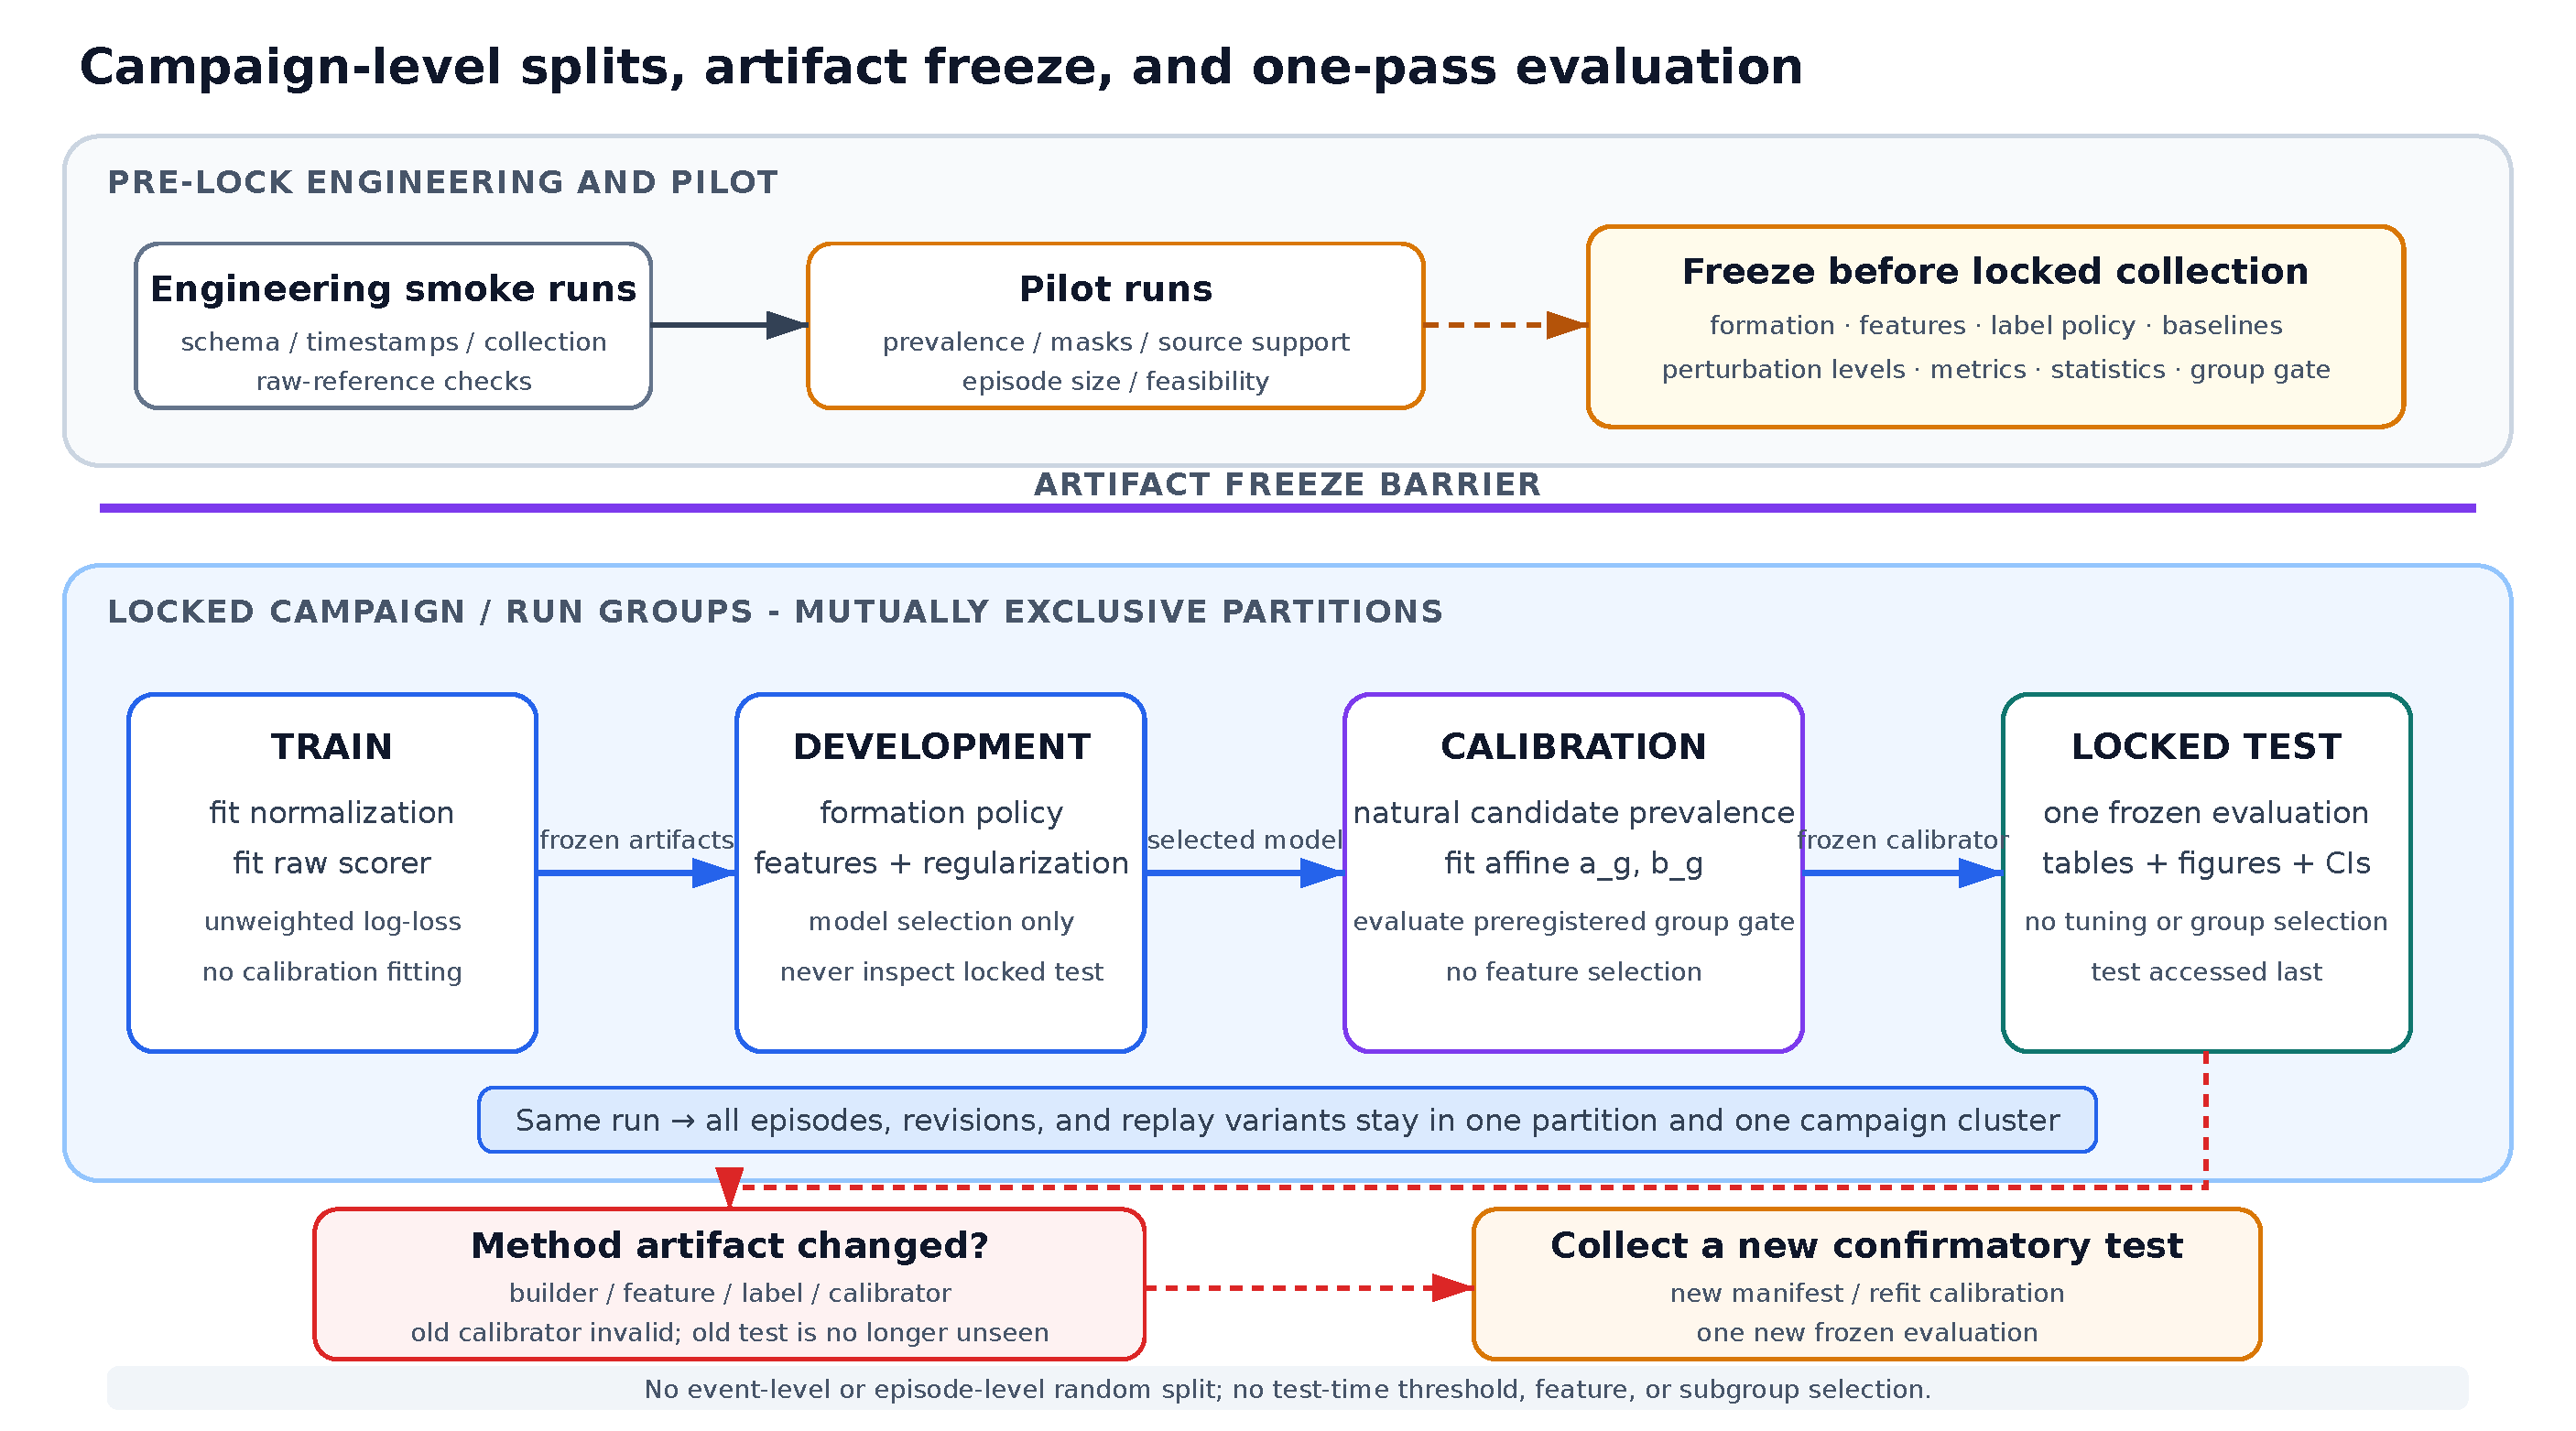
\includegraphics[width=\textwidth]{trustepisode_figures/pdf/fig06_split_and_freeze_workflow.pdf}
  \caption{Campaign-level split and freeze workflow. Deterministic 50/20/15/15 assignment is
  performed before label release, and all descendants inherit the base campaign partition and
  bootstrap cluster.}
  \label{fig:split-freeze-companion}
\end{figure*}

\subsection{Baseline Implementation Registry}

EB1 uses non-overlapping event-time windows of width $W_{\mathrm{gap}}$ with no entity or
causal merge. EB2 adds the requirement that consecutive records share one specific,
non-generic entity. EB3 is Algorithm~1; EB3-H changes only hub suppression. SB1 is the maximum
source-normalized vendor severity among eligible episode records. SB2 fits the same constrained
logit procedure as Equation~\ref{eq:raw-logit} with $w_C=0$. SB3 is the proposed raw logit.
SB4 reports the uncalibrated sigmoid score $\sigma(z)$ and is not called a probability. SB5
applies the global affine calibrator. SB6 is the
conditional group mapping. SB7 maps an unavailable source's absent detector value to zero and
ignores manifest support. OB1 is the physical-outage-only available-source denominator and
returns no corroboration when fewer than two source families are healthy. No entry has an
alternative max/mean, weight set, model capacity, or post-test implementation.

\subsection{Frozen Perturbation Grid and Outage Procedure}

\begin{table*}[t]
\caption{Pre-registered replay perturbations. Each variant includes an unchanged control and
uses a deterministic child seed derived from the base-run ID.}
\label{tab:perturbation-grid}
\centering
\small
\begin{tabular}{p{0.08\textwidth}p{0.21\textwidth}p{0.27\textwidth}p{0.33\textwidth}}
\toprule
\textbf{ID} & \textbf{Intervention} & \textbf{Frozen levels} & \textbf{Invariant} \\
\midrule
RP0 & unchanged replay & no mutation & exact canonical-hash equality required \\
RP1 & source-event mask & EDR only; NDR only & SourceCoverage unchanged \\
RP2 & independent random drop & 5\%; 10\%; 25\% & retained event times and health unchanged \\
RP3 & bounded burst drop & 30 s; 120 s; 300 s & one seeded interval per run \\
RP4 & ingest delay & 30 s; 120 s; 600 s & event time unchanged \\
RP5 & arrival reorder & buffer of 30 s; 120 s; 600 s & payload and event time unchanged \\
RP6 & event-time clock skew & $-120$; $-30$; $+30$; $+120$ s & ingest time and health unchanged \\
RP7 & dependency-aware duplicate & 5\%; 10\%; 25\% & duplicate retains root dependency group \\
\bottomrule
\end{tabular}
\end{table*}

Every replay child seed is HMAC-SHA256 over base-run ID, intervention, and level with key
\texttt{20260710}; descendants retain the base label, split, and cluster. The exact registry is
\path{artifacts/contracts/perturbations.v1.json}.

Physical outage uses the same scenario/seed pair as a normal run. After a 120-second steady
state, the selected EDR or NDR collector is stopped or network-isolated for 120 or 600 seconds,
then restored. The procedure records last healthy heartbeat, first degraded/down
SourceCoverage interval, watermark movement, emitted revisions, $\kappa$, eligibility,
recovery heartbeat, and stable revision. Recovery requires two healthy heartbeats, a valid
parser, backlog no greater than 120 s, and no new revision for 900 s. Safety aborts the run if
isolation affects the control plane or a non-laboratory route.

\subsection{Matching and Metric Formulas}

Before primary assignment, a $\mathcal C_{form}$ terminal revision is match eligible only with
temporal IoU at least $.10$, entity Jaccard at least $.50$, and one exact marker or registered
action. For eligible pairs,
\begin{equation}
w=.5A_{cov}+.3J_{entity}+.2\operatorname{IoU}_{time};\qquad
w\ge\theta_{match}=.50.
\end{equation}
Maximum-weight bipartite assignment operates within one run; ties use greater entity overlap,
smaller absolute time difference, then lexical IDs. Formation metrics use $\mathcal C_{form}$,
ranking and calibration use $\mathcal C_{dec}$, and only transition/cost analyses use
$\mathcal C_{stream}$.

For ground-truth malicious-action set $A$ and the actions covered by assigned revisions
$\widehat A$,
\begin{equation}
\mathrm{ActionCoverage}=\frac{|A\cap\widehat A|}{|A|}.
\end{equation}
For run $r$, let $G_r$ be its ground-truth action groups and $n_g$ the number of distinct
terminal predicted episodes assigned to group $g$. Fragmentation is
$|G_r|^{-1}\sum_{g\in G_r}\max(0,n_g-1)$. Over-merge is the fraction of terminal predicted
episodes assigned to more than one distinct action group in the same run; the unit is never a
mutually exclusive run ID. Benign contamination is the fraction of unrelated benign events
inside revisions assigned to malicious groups. Episode precision, recall, and F1 use the
locked one-to-one assignment.

For supported records $i=1,\ldots,n_{\mathrm{sup}}$,
\begin{align}
\mathrm{Brier}&=\frac{1}{n_{\mathrm{sup}}}\sum_i(P_i-Y_i)^2,\\
\mathrm{NLL}&=-\frac{1}{n_{\mathrm{sup}}}\sum_i
[Y_i\log P_i+(1-Y_i)\log(1-P_i)].
\end{align}
Out-of-support records are absent from both sums. Reliability uses ten fixed equal-width bins
on $[0,1]$ and always reports bin counts. Supported decision coverage is
$|\mathcal C_{\mathrm{sup}}|/|\mathcal C_{dec}|$. Ranking reports AUPRC and recall among the
top $\max(1,\lceil0.05|\mathcal C_{dec,r}|\rceil)$ revisions in each run; AUROC and precision
at the same budget are secondary. All primary summaries are run-macro means; pooled micro
results are supplemental.

\subsection{Run-Level Uncertainty and RQ Matrix}

Primary intervals use 2,000 cluster-bootstrap resamples of complete campaign/run clusters with
seed 20260710 and percentile endpoints at 2.5\% and 97.5\%. For paired replay and outage
contrasts, the resampled object is the base-run pair. A resample lacking both classes for a
class-dependent metric is marked undefined for that metric and counted; it is not replaced by
zero. Run-level p50/p95/p99 latency and throughput are computed before cross-run aggregation.

\begin{table*}[b]
\caption{Frozen RQ--comparison--metric matrix.}
\label{tab:rq-matrix}
\centering
\small
\begin{tabular}{p{0.09\textwidth}p{0.31\textwidth}p{0.31\textwidth}p{0.19\textwidth}}
\toprule
\textbf{RQ} & \textbf{Comparison/intervention} & \textbf{Primary outcomes} & \textbf{Unit} \\
\midrule
RQ1 & EB1, EB2, EB3, EB3-H & action coverage; fragmentation; over-merge & campaign/run \\
RQ2 & SB1--SB5; SB6 conditional & AUPRC; fixed-budget recall; Brier; NLL; reliability & campaign/run \\
RQ3 & paired replay grid; separate outage pairs & formation/$z$/support/$U$/revision changes; outage detection/recovery & base-run pair \\
RQ4 & unchanged replay; frozen hardware run & canonical digest equality; throughput; latency; memory; storage; replay time & campaign/run \\
\bottomrule
\end{tabular}
\end{table*}

\subsection{Result Registry and Canonical Replay}
\label{app:result-shells}

RT1 contains split, population, run, candidate, positive, negative, mixed, ambiguous, and
prevalence counts. RT2 contains formation metrics. RT3a contains ranking comparators; RT3b
contains supported calibration only. RT4 contains paired replay effects. RT5 contains physical
outage and recovery, including OB1. RT6 contains determinism and resource cost. RT7 contains
registered error categories. Every unexecuted cell is serialized as \texttt{pending}, never
zero; \texttt{N/A} is reserved for structurally inapplicable fields. The machine schema is
\path{artifacts/contracts/result_registry.v1.json}.

\begin{table*}[t]
\caption{RT3a ranking-result shell. SB1 has no probability mapping.}
\label{tab:ranking-results}
\centering
\small
\begin{tabular}{lcccc}
\toprule
\textbf{Scorer} & \textbf{AUPRC} $\uparrow$ & \textbf{Recall@budget} $\uparrow$ & \textbf{AUROC} $\uparrow$ & \textbf{Precision@$k$} $\uparrow$ \\
\midrule
SB1 static severity & \tbd & \tbd & \tbd & \tbd \\
SB2 $D$ only & \tbd & \tbd & \tbd & \tbd \\
SB3 $D+C$ raw & \tbd & \tbd & \tbd & \tbd \\
\bottomrule
\end{tabular}
\end{table*}

\begin{table*}[t]
\caption{RT3b calibration-result shell over supported records only.}
\label{tab:calibration-results}
\centering
\small
\begin{tabular}{lccccc}
\toprule
\textbf{Mapping} & \textbf{Brier} $\downarrow$ & \textbf{NLL} $\downarrow$ & \textbf{Reliability} & \textbf{Supported coverage} & \textbf{Out-of-support rate} \\
\midrule
SB4 uncalibrated sigmoid score & \tbd & \tbd & pending & \tbd & \tbd \\
SB5 supported global & \tbd & \tbd & pending & \tbd & \tbd \\
SB6 supported group & \tbd & \tbd & pending & \tbd & \tbd \\
\bottomrule
\end{tabular}
\end{table*}

The RQ4 canonical payload consists of episode and revision IDs, ordered event membership,
link reasons, $D,C,a^{det},z,P,\kappa,U$, detector and health states,
\texttt{decision\_eligible}, versions, policy and artifact hashes, and evidence references.
Equality is byte-for-byte SHA-256 equality under
Appendix~\ref{app:canonical-serialization}. Execution timestamps and host-specific runtime
metadata are excluded from this claim.

The formal machine contracts and this expanded appendix are packaged as
\path{TrustEpisode_reproducibility_companion_v1.zip}; the adjacent \path{.sha256} sidecar
authenticates the exact distributed bytes. The bundle contains no fabricated runs or results.
